% !TEX root=../presentation_1.tex
\section{Introduction}

\subsection{Minimum-Weight Spanning Tree (MST)}

\begin{frame}
\frametitle{Minimum-Weight Spanning Tree (MST)}

\begin{itemize}
  \item A \textbf{weighted} graph $G = (V,E,W)$.
  \item A \textbf{spanning tree} is a tree that covers all vertices.
  \item A spanning tree is \textbf{minimum} if the sum of all weights in the tree is the minimum among all spanning trees.
\end{itemize}
\begin{figure}
    \centering
    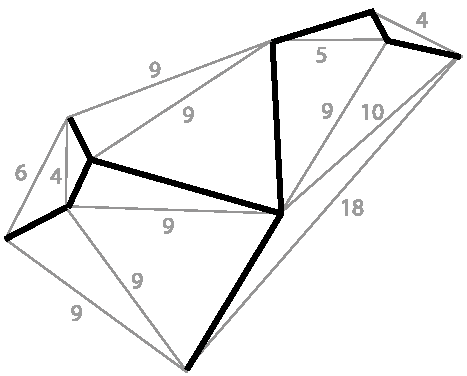
\includegraphics[width=0.4\textwidth]{figures/mst.pdf}
    \caption{An example of MST}
\end{figure}
\end{frame}

\subsection{Greedy Sequential Algorithms}

\begin{frame}
\frametitle{Greedy Sequential Algorithms}

\begin{itemize}
% \item \textcolor{red}{\textbf{Red}} rule. Heaviest edge in a cycle is not in the MST.
% \item \textcolor{blue}{\textbf{Blue}} rule. 
\item Lightest edge across a cut is in the MST.
\end{itemize}
\begin{itemize}
  \item Kruskal's algorithm
    \begin{itemize} 
      \item Adding the minimum weighted edge without forming a cycle.
    \end{itemize}
  \item Prim's algorithm
    \begin{itemize} 
      \item Expanding by selecting the minimum weighted outgoing edge.
    \end{itemize}
  \item Boruvka's algorithm
    \begin{itemize}
      \item Locally merging components by picking the minimum weighted edge connecting both components.
    \end{itemize}
\end{itemize}
\end{frame}

% \begin{frame}
% \begin{figure}
%     \resizebox{.48\textwidth}{!}{
% \animategraphics{12}{figures/KruskalDemo-}{0}{92}
% }
%     \resizebox{.48\textwidth}{!}{
% \animategraphics{12}{figures/PrimAlgDemo-}{0}{57}
% }
% \caption{Left: Kruskal's Algorithm; Right: Prim's Algorithm}
% \end{figure}
% \end{frame}